%%
%% forked from https://gits-15.sys.kth.se/giampi/kthlatex kthlatex-0.2rc4 on 2020-02-13
%% expanded upon by Gerald Q. Maguire Jr.
%% This template has been adapted by Anders Sjögren to the University
%% Engineering Program in Computer Science at KTH ICT. Adaptation is the
%% translation of English headings into Swedish as the addition of Swedish
%% text. Original body text is deliberately left in English.


%% set the default lanage to english or swedish by passing an option to the documentclass - this handles the inside tile page
\documentclass[english]{kththesis}
%\documentclass[swedish]{kththesis}

% \usepackage[style=numeric,sorting=none,backend=biber]{biblatex}

\setlength {\marginparwidth }{2cm} %leave some extra space for todo notes
\usepackage{todonotes}

\usepackage[perpage,para,symbol]{footmisc} %% use symbols to ``number'' footnotes and reset which symbol is used first on each page

%% Reduce hyphenation as much as possible
\hyphenpenalty=15000 
\tolerance=1000

%%----------------------------------------------------------------------------
%%   pcap2tex stuff
%%----------------------------------------------------------------------------
%\usepackage[dvipsnames*,svgnames]{xcolor} %% For extended colors
\usepackage{tikz}
\usetikzlibrary{arrows,decorations.pathmorphing,backgrounds,fit,positioning,calc,shapes}
\usepackage{pgfmath}	% --math engine

%% some additional useful packages
\usepackage{rotating}		%% For text rotating
\usepackage{array}		%% For table wrapping
\usepackage{graphicx}	        %% Support for images
\usepackage{float}		%% Suppor for more flexible floating box positioning
\usepackage{mdwlist}            %% various list-related commands
\usepackage{setspace}           %% For fine-grained control over line spacing
\usepackage{listings}		%% For source code listing
\usepackage{bytefield}          %% For packet drawings
\usepackage{tabularx}		%% For simple table stretching
\usepackage{multirow}	        %% Support for multirow colums in tables

\usepackage{url}                %% Support for breaking URLs
\usepackage{hyperref}
\usepackage[all]{hypcap}	%% prevents an issue related to hyperref and caption linking
%% setup hyperref to use the darkblue color on links
\hypersetup{colorlinks,breaklinks,
            linkcolor=darkblue,urlcolor=darkblue,
            anchorcolor=darkblue,citecolor=darkblue}

\makeatletter
\setlength{\@fptop}{0pt}
\setlength{\@fpbot}{0pt}
\makeatother

%% Some definitions of used colors
\definecolor{darkblue}{rgb}{0.0,0.0,0.3} %% define a color called darkblue
\definecolor{darkred}{rgb}{0.4,0.0,0.0}
\definecolor{red}{rgb}{0.7,0.0,0.0}
\definecolor{lightgrey}{rgb}{0.8,0.8,0.8} 
\definecolor{grey}{rgb}{0.6,0.6,0.6}
\definecolor{darkgrey}{rgb}{0.4,0.4,0.4}
\definecolor{aqua}{rgb}{0.0, 1.0, 1.0}

%% If you are going to include source code (or code snippets)
\usepackage{listings}
%%\usepackage[cache=false]{minted} %% For source code highlighting
%%\usemintedstyle{borland}

\usepackage{csquotes} % Recommended by biblatex


%% Acronyms
% note that nonumberlist - removes the cross references to the pages where the acronym appears
% note that nomain - does not produce a main gloassay, this only acronyms will be in the glossary
% note that nopostdot - will present there being a period at the end of each entry
\usepackage[acronym, section=section, nonumberlist, nomain, nopostdot]{glossaries}
%\glsdisablehyper
\makeglossaries
%%% Local Variables:
%%% mode: latex
%%% TeX-master: t
%%% End:
\newacronym{NFV}{NFV}{Network Function Virtualization}
\newacronym{NF}{NF}{Network Function}
\newacronym{SDN}{SND}{Software Defined Networking}
\newacronym{VM}{VM}{Virtual Machine}
\newacronym{HPC}{HPC}{High Performance Computing}
\newacronym{DPDK}{DPDK}{Data Plane Development Kit}
\newacronym{OS}{OS}{Operating System}
\newacronym{UIO}{UIO}{User space Input/Output}
\newacronym{NIC}{NIC}{Network Interface Controller}
\newacronym{PMD}{PMD}{Poll Mode Driver}
\newacronym{EAL}{EAL}{Environment Abstraction Layer}
\newacronym{NAT}{NAT}{Network Address Translation}

\newacronym{LAN}{LAN}{Local Area Network}
\newacronym{WLAN}{WLAN}{Wireless Local Area Network}
\newacronym{UN}{UN}{United Nations}
\newacronym{SDG}{SDG}{Sustainable Development Goal}
\newacronym{TLB}{TLB}{Translation Lookaside Buffer}
                %load the acronyms file

%% definition of new command for bytefield package
\newcommand{\colorbitbox}[3]{%
	\rlap{\bitbox{#2}{\color{#1}\rule{\width}{\height}}}%
	\bitbox{#2}{#3}}

%% a bit higher line width in tables
\renewcommand{\arraystretch}{1.3}

% to find unicode characters that LaTeX complains about
\DeclareUnicodeCharacter{F0DE}{XXXX Here I am?????XXXX}

\newenvironment{swedishnotes}%
  {\begin{center}
      \selectlanguage{swedish}
      \color{blue}}%
    {\end{center}
    \selectlanguage{USenglish}}
    
\lstnewenvironment{code}[1][]%
  {\noindent\minipage{\linewidth}\medskip 
   \lstset{basicstyle=\ttfamily\footnotesize,frame=single,#1}}
  {\endminipage}    

\graphicspath{{figures/}}

\usepackage{afterpage}
\newcommand\blankpage{%
    \null
    \thispagestyle{empty}%
    \addtocounter{page}{-1}%
    \newpage}

\begin{document}
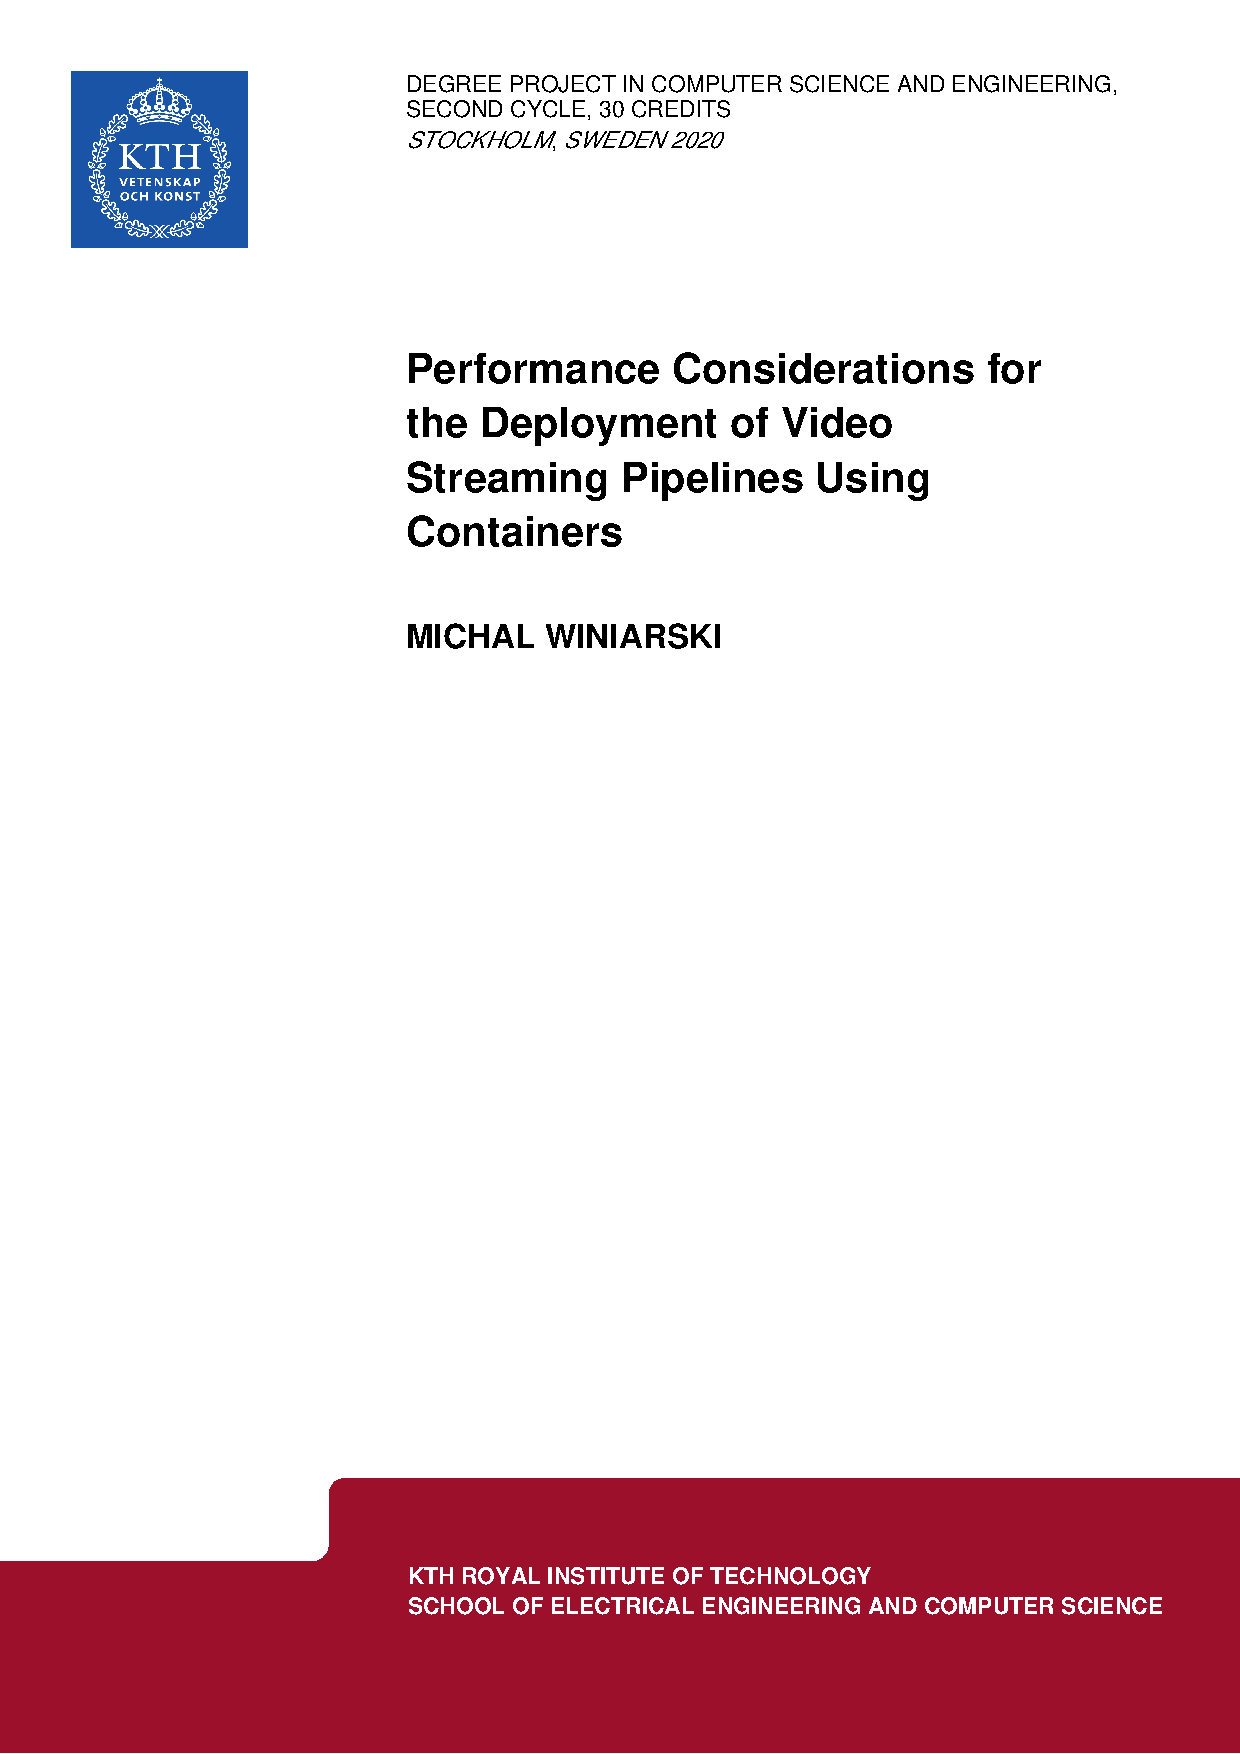
\includepdf[pages={1}]{cover.pdf}
\afterpage{\blankpage}
\selectlanguage{USenglish}
%\selectlanguage{UKenglish}
%\selectlanguage{english}
%\selectlanguage{swedish}

%% Information for inside title page
\title{Performance Considerations for the Deployment of Video Streaming Pipelines Using Containers}
%\subtitle{An subtitle in the language of the thesis}

% give the alternative title - i.e., if the thesis is in English, then give a Swedish title
\alttitle{Prestationsöverväganden vid distribution av videoströmningsrörledningar med behållare}
%\altsubtitle{Detta är den svenska översättningen av undertiteln}

\author{Michał Winiarski}
\email{michalwi@kth.se}

\supervisor{Sladjana Josilo}
\examiner{György Dán}
\hostcompany{Net Insight} % Remove this line if the project was not done at a host company
\companysupervisor{Jonas Nordqvist}

\date{\today}

\programcode{TCOMM}
%% Alternatively, you can say \programme{Civilingenjör Datateknik} to directly set the programme string

\schoolAcronym{EECS}
%% Alternatively, you can say \school{School of Electrical Engineering and Computer Science} to directly set the school string

\titlepage
% document/book information page
\bookinfopage

% Frontmatter includes the abstracts and table-of-contents
\frontmatter
\setcounter{page}{1}
\begin{abstract}
\markboth{\abstractname}{}
Cloud-based video processing is an area depending heavily on the hardware's ability to process huge amounts of packets. Nowadays, we can observe industry drifting away from commonly used FPGAs in lieu of a more flexible software approach. Docker container has been considered a promising technology for constructing video streaming pipelines as it provides a fast and easy way to package and distribute software.
Recent developments in the Network Function Virtualization field showed that fast packet processing frameworks like Intel \gls{DPDK} have a potential to improve the performance of network function chains. This technology could be an enabler for software video processing to approach hardware solutions, yet it is still in quite an early stage and generates many questions about usage, deployment, and performance. 

This thesis shows that it is possible to build packet processing pipelines using DPDK, running dozens of video processing microservices simultaneously on a single machine. The project implementation was evaluated in terms of latency and throughput and behaviour of co-running applications on a single CPU core was modelled.

\subsection*{Keywords}
Streaming media, Docker, NFV, DPDK, Multithreading

\end{abstract}
\cleardoublepage
\begin{otherlanguage}{swedish}
  \begin{abstract}
    \markboth{\abstractname}{}
Molntjänster Inom området videobearbetning är starkt beroende av hårdvarans förmåga att kontinuerligt  bearbeta mycket stora mängder paket. Idag har det blivit vanligt inom professionell användning att välja bort tidigare vanliga FPGA-baserade lösningar, till förmån för mer flexibla mjukvarubaserade lösningar. Docker containers har setts som en lovande teknologi för att konstruera pipelines för strömmande video, då de erbjuder ett snabbt och enkelt sätt att paketera och distribuera mjukvara.

Utvecklingen inom virtualisering av nätverksfunktioner (NFV) har visat att ramverk för snabb paketprocessning, såsom Intel DPDK, har potential att förbättra prestandan hos kedjor av nätverksfunktioner. Denna teknologi gör det möjligt för mjukvarubaserad videobehandling att hävda sig i jämförense med hårdvarubaserade varianter. Den är dock relativt ny och oprövad och det kvarstår många öppna frågor om användning, driftsättning och prestanda.

Detta examensarbete visar att det är möjligt att bygga paketbearbetande pipelines med DPDK, som kör dussintals nätverksfunktioner samtidigt på en maskin. En implementation har konstruerats och utvärderats med fokus på latens och flöde, och beteendemönster för applikationer som kör samtidigt på samma CPU har modellerats.
\subsection*{Nyckelord}
Strömmande media, Docker, NFV, DPDK, Multitrådning


  \end{abstract}
\end{otherlanguage}
\cleardoublepage
\section*{Acknowledgments}
I would like to express my gratitude to my thesis examiner György Dán for giving me the opportunity to write this thesis and to my supervisor Sladjana Josilo for all the great work she put into revisions.\\
I would also like to thank Jonas Nordqvist and Rickard Molin at Net Insight AB for guidance and supervision on the project and for allowing me to work under the company's patronage.
\markboth{Acknowledgments}{}

\acknowlegmentssignature

\fancypagestyle{plain}{}
\renewcommand{\chaptermark}[1]{ \markboth{#1}{}} 
\tableofcontents
  \markboth{\contentsname}{}

\cleardoublepage

%\listoffigures
%\cleardoublepage

%\listoftables
%\cleardoublepage

%\lstlistoflistings\todo{If you have listings in your thesis.}
%\cleardoublepage

%\printglossary[type=\acronymtype, title={List of acronyms and abbreviations}]
%\todo[inline]{The list of acronyms and abbreviations should be in alphabetical order based on the spelling of the acronym or abbreviation.}

\label{pg:lastPageofPreface}
% Mainmatter is where the actual contents of the thesis goes
\mainmatter

\renewcommand{\chaptermark}[1]{\markboth{#1}{}}
\chapter{Introduction}
\label{ch:introduction}
Multimedia content such as video traffic has been rapidly increasing over the past years. According to a recent estimate by Cisco, 79\% of the world's mobile data traffic will be video by 2022 \cite{cisco}. The increasing demand for video content puts pressure on the live media industry that needs to find new media streaming solutions in order to meet user requirements. Recently, with the advent of \gls{SDN} and \gls{NFV}, the networking industry started moving its products from specialized video hardware into the cloud infrastructure. This movement enables faster development and decreases costs, but it also puts more pressure on the software efficiency \cite{intro}. One of the premises of this cloud approach is to break down the usually monolithic, complicated functionality of the network management software into separate network functions. Initially, the software would be split into several  \glspl{VM}. However, it is not feasible to run high amount of \glspl{VM} on a single hardware due to the fact that each of them needs to run a separate operating system. That is where a container, the OS-level virtualization technique, becomes important. 

Linux container realm, lead undisputed by Docker (79\% of all containers are Dockers), is now a widely used and mature technology \cite{docker_stats}. By exploiting features like namespaces and cgroups it provides much-needed features in the software industry: flexibility, scalability, and isolation. It makes an ideal choice for implementing video pipelines, which usually come in form of chains of several interconnected Linux applications processing UDP streams. Various offline \gls{HPC} applications like genomic pipelines, deep learning algorithms, or gaming servers have been tested to prove containerization software produces negligible overheads in CPU consumption. However, it has been shown that using containers can impact network performance, which is not an obstacle for offline tasks, but is very important for tasks involving packet processing that depend on latency.

Packet processing using commodity hardware puts very high demand on software, which results in the operating system being the bottleneck. In order to address this problem, \gls{NFV} industry proposed userspace packet processing method that optimizes the way Linux network stack processes packets. This method has gained increasing popularity as it allows the developers to fully take packet processing in their hands, without having to be concerned about overheads of the operating system.

This thesis presents a solution in the form of a framework being able to set up considerable amounts of containerized network functions exploiting kernel bypass techniques for inter-process communication and producing broad network statistics about their performance. The idea behind the kernel bypass is to remove the kernel from the packet processing stack, allowing packets to be received from hardware directly into the userspace. A widely accepted framework providing said functionality is Intel's \gls{DPDK}. It offers a set of tools useful for fast packet processing, like I/O batching and memory queues for packet handling.

%We use the \emph{bibtex} package to handle our references.  We therefore
%use the command \cite{farshin_make_2019}. For example, Farshin, et al. described how to improve LLC
%cache performance in \cite{farshin_make_2019} in the context of links running
%at \SI{200}{Gbps}.

\section{Overview}
\label{sec:background}
This section aims to describe a simplified version of the common product in the media industry, on which this thesis is based on. The product is a middle-box, built with common hardware and running Linux OS. Inside there is a management system that is responsible for the administration of applications performing different media and network functions. Examples of such programs are video encoders and decoders, network monitoring, traffic encryption, re-transmission software, or firewall. In most cases, the video being processed is input on a network or video interface and passes through a chain of consecutive programs in the form of a UDP stream. In the end, it is output on another network interface. Commonly, many identical processing pipelines start and terminate at the same interfaces, and a system in general must be able to support up to 10 Gigabits of network traffic. An example of simplified system running on top of Linux OS is shown in Figure~\ref{fig:commonsetup}. As illustrated in the figure, the system must be able to support multiple applications running simultaneously (up to a few dozens in the real systems).

\begin{figure}[!ht]
  \centering
    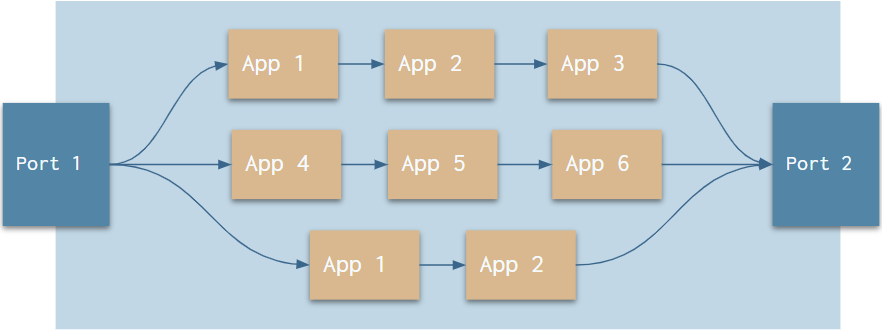
\includegraphics[width=1\textwidth]{Fig1}
  \caption{Common video processing setup. The figure presents a simplified system running on top of Linux based OS.}
  \label{fig:commonsetup}
\end{figure}

\section{Motivation and challenges}
\label{sec:motivation}
In live-video processing, there are strict requirements on the packet’s latency in the network as well as on throughput. If the application introduces latency to the packets, then it has to be stabilized by the receiver’s queue, which in turn adds to the latency. High CPU consumption, as well as low throughput, can decrease the maximum number of streams that could be run on the machine. Altogether it is a difficult task to maintain a good quality of service while keeping in mind its cost-effectiveness.

Considering the scenario presented in the previous section there are two main requirements that need to be satisfied. Firstly, the system must be very efficient in terms of CPU consumption by itself. Secondly, the user of the system must be able to make an informed decision (manual or automatic) based on each application, pipeline, and CPU core individual performances.

The purpose of this thesis is to provide an insight into the usage of fast packet processing techniques for containerization software to improve the efficiency and quality of the product sold by the principal of this thesis. It should also provide the implementation of state of the art tooling. Finally, it should provide some insights into the buzzing areas of cloud computing and \gls{NFV}, and support the academy and engineering community with its results.

The main goal of this project is to improve cloud video processing performance. This goal consists of the following sub-goals: 

\begin{enumerate}
\item Investigate Docker container networking and identify its caveats.
\item Implement fast packet processing between containers using \gls{DPDK}.
\item Formulate a model that describes system behaviour.
\item Collect measurements to verify the model and draw conclusions.
\end{enumerate}

\section{Research methodology}
An in-depth study of Docker containers and \gls{DPDK} fast packet processing was done. Based on the conducted study a framework solution was proposed and implemented. The outcome was then tested in different setups regarding applications' CPU core affinity, count of chains and applications, their workload, and thread switching frequency. Results were evaluated in terms of system throughput, latency, and CPU usage. The different steps followed in this research method are:
\begin{enumerate}
    \item Literature Study
    \item Experimental design and implementation
    \item System modeling
    \item Data collection and analysis
\end{enumerate}

Although the purpose of this thesis is to allow improving the methods and applications used in the industry, this work does not use real-world applications to perform the tests on. The reason for that is that transforming and debugging industry-level programs would require vast amounts of work. Instead stub programs are used to simulate real workloads which allow for a better understanding of the processes and underlying performance.

\section{Thesis structure}
The structure of this thesis is as follows. Chapter~\ref{ch:background} presents relevant background information about fast packet processing and containers. Chapter~\ref{ch:methods} presents the methodology and method used to solve the problem. Chapter~\ref{ch:whatYouDid} presents the model of the system and implementation. Chapter~\ref{ch:resultsAndAnalysis} presents the results and talks about their interpretation.  Chapter~\ref{ch:conclusionsAndFutureWork} talks about the conclusion and future works.

\section{Sustainability and ethical concerns}
The main area of focus for this project is network optimization. It aims to help engineers build more efficient systems, hence reducing the energy consumption required to perform certain amount of computation. Regarding ethical concerns, this thesis does not use any of the principal company's confidential data or intellectual property.

\cleardoublepage
\chapter{Background}
\label{ch:background}
This chapter describes the crucial information the reader needs to understand this thesis. It begins by describing the utilization of containers and diving into the Docker specifics. Then it describes the area of network optimization and introduces specific tools used in this work.

\section{Containers}
A container is known as OS-level virtualization technology. Its purpose is to package software together with dependencies and provide isolation from other processes running on the same machine \cite{what_is_container}. The containers share the kernel and resources of the host OS, which also gives them several advantages (e.g., better CPU and memory performance, lesser volume) when compared to running the software on separate \glspl{VM}.

The need for using \gls{VM} comes from the need of software isolation. It is often unwanted to allow applications running on the same machine to share network, access to files, or processes. Containers allow developers to deploy many programs on the same system without the problems related to the same IP or port pools, or access to different library dependencies \cite{container_usage}. This is achieved using a technology called namespaces \cite{namespaces}. Another technology useful for managing containers is Linux's control groups - cgroups \cite{cgroups}. They allow developers to limit and monitor how resources like CPU and memory are used by a group of programs.

For developers, this means that the total isolation of processes running on one machine can be achieved without the usage of expensive hypervisors and \glspl{VM}. This results in saving large amounts of resources. Furthermore, while starting a virtual machine can take up to minutes, a container can be spun up in a matter of milliseconds. Consequently, containers have been seen as promising tools for fast testing and deployment, and hence for enabling dynamic run-time management of containerized software. The architectural differences between containers and virtual machines are presented in Figure~\ref{fig:containerVM}. As illustrated in the figure, the main difference is usage of operating system - separate for each application instance of virtual machine, and shared between applications using containers.

\begin{figure}[!ht]
  \centering
    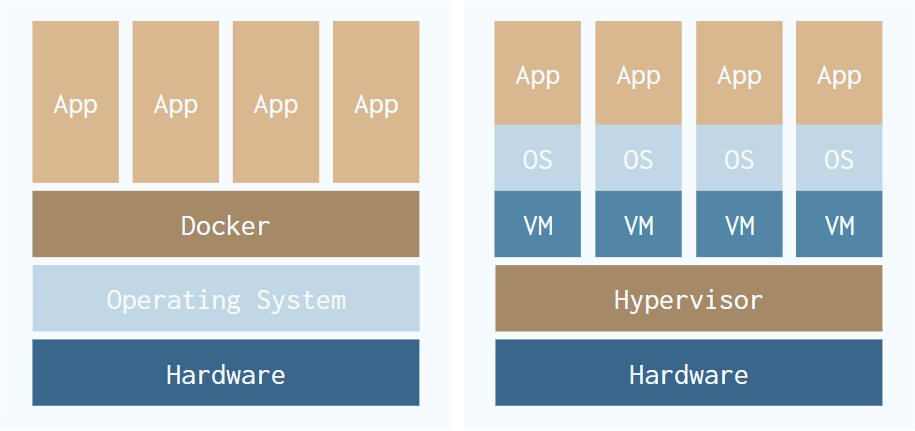
\includegraphics[width=1\textwidth]{Fig2}
  \caption{Containers vs. Virtual Machines}
  \label{fig:containerVM}
\end{figure}

\subsection{Docker architecture}
Docker has been recognized as a platform leading in the container industry. It can be described as a complex system with various out of the box solutions for building software images, running containers, managing networks, and many others. There are two aspects important for this thesis regarding the working of Docker: networking and bind mounts.

\subsubsection{Networking}
Networking is a very powerful aspect of the Docker platform allowing various configurations of connectivity between containers. Docker exploits features available in Linux networking like namespaces, bridges, veth pairs, and iptables \cite{docker_networking}. There are 5 different network drivers that Docker users can choose from:
\begin{itemize}
    \item bridge - default and most common network driver allowing communication between containers on the same operating system,
    \item host - allows programs inside the containers to be treated like they would be running on the host and share the port pool,
    \item macvlan - allows assigning MAC address to the container, making it appear as a physical device on the network,
    \item overlay - used when many Dockers on multiple hosts need to communicate,
    \item none - disables container's communication with the host.
\end{itemize}

When thinking about connecting dozens of standalone containers there are three suitable candidates: Linux bridge, macvlan, and host. Bridge is the best candidate when it comes to management. It allows for very needed dynamic IP address and port assignments and would let different pipelines to be isolated by distinct bridges. However, bridges suffer from the following problems. First, Linux bridge is a software switch, which has an impact on network latency as every packet entering or leaving a container must be routed by the Linux network stack. Second, packets routed in and out of a bridge are subject to NAT routing which also has slight impact on performance \cite{anderson_2016}. An example of bridge driver concept is shown in Figure~\ref{fig:bridge}.

\begin{figure}[!ht]
  \begin{center}
    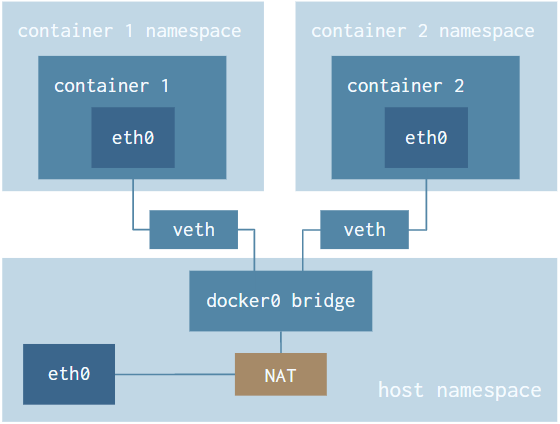
\includegraphics[width=0.8\textwidth]{Fig3}
  \end{center}
  \caption{Docker bridge network driver}
  \label{fig:bridge}
\end{figure}

Macvlan networks are mostly used with legacy applications. They can be useful when there is a requirement for the container to be directly connected to the physical network. \cite{anderson_2016} shows that macvlans can outperform bridges in terms of latency. However, there are few disadvantages related to using them like IP address exhaustion and VLAN spread - a problem arising with a large number of MAC addresses in the network \cite{macvlan}.

Finally, different from bridge and macvlan, the host mode does not suffer from the problems related to extra software switching or NAT as in this case containers share the network namespace with the host \cite{host}. However, even simply using the Linux OS networking for inter-process communication increases packets transferred between programs' latency as they must pass through the network stack.

\subsubsection{Bind mounts}
In Docker bind mounts can be used to mount a file or directory on the host machine into a container \cite{bind_mounts}. By default, Docker containers have isolated file systems as well as restricted access to shared memory (mnt and ipc namespaces). To provide an alternative to network communication containers must be explicitly instructed to either join the same ipc namespace or mount the same folder from the host's file system. The latter is the technique used to share the hugepage resources managed by the \gls{DPDK}.

\section{Fast packet processing}
This section describes what improvements can be made to a system to improve packets processing, where the requirements come from, and what underlying mechanisms take part in the process.

\subsection{Network function virtualization}
\gls{NFV} is a fairly recent paradigm in the communications systems area. The key idea of NFV is to move the implementation of network nodes from dedicated hardware into the common computers so as to increase the agility, and thus to allow for quick changes in the infrastructure \cite{nvf_redhat}. This approach not only brings the power of fast deployment, updates, scalability, and agile development but can also significantly reduce costs. The disadvantage of the departure from dedicated hardware, however, is the decrease in overall performance of the system, putting pressure mostly on its networking capabilities. When creating software for \gls{NFV} not only must the Network Functions themselves be highly efficient, but also the underlying network stack, as all the low-level parts like CPU core affinity, scheduling, cache locality, or synchronization may greatly influence its performance. To allow easier research and development of these details the implementation of packet processing has shifted into the userspace. The general-purpose Linux kernel proved itself to not be efficient and flexible enough.

\subsection{Userspace packet processing}
\label{userspace_pp}
In this section, the focus is on the packet processing techniques that allow for improving the system efficiency in terms of throughput and latency: kernel bypass, zero-copy, and I/O packet batching.

\subsubsection{Kernel bypass}
Modern \glspl{OS} provide a wide range of networking functionalities, such as packet handling, routing, filtering \cite{packet_receiving_2007}. Furthermore, in order to manage various types of protocols, the kernel implementation operates on many different abstractions. This generality may come with a performance cost when compared to solutions created specifically for a single scenario, and for some solutions, like software router, the network stack is not even needed \cite{barbette_2015}. Linux example software networking stack is presented in Figure~\ref{fig:softstack}.
\begin{figure}[!ht]
  \begin{center}
    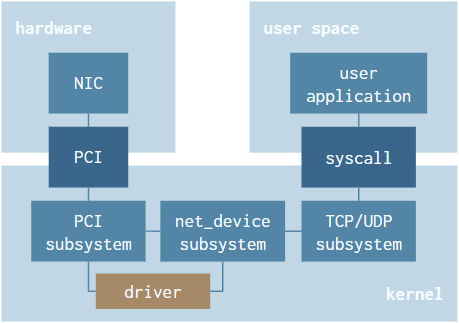
\includegraphics[width=0.8\textwidth]{Fig4}
  \end{center}
  \caption{Example of Linux networking software stack. Today, the most commonly used interface for communication between kernel drivers and network devices is a PCI bus, e.g., PCI Express.}
  \label{fig:softstack}
\end{figure}
Bypassing the parts of the kernel where packet processing is performed can be achieved by directly accessing the PCI subsystem. This feature is provided by the \gls{UIO} kernel module (driver), which exposes a set of files for each Ethernet device, which the user-space applications can interact with \cite{codilime}.

\subsubsection{Zero-copy}
When receiving data in standard networking stack the packet is firstly copied from the \gls{NIC} into kernel buffers. Then, after a system call from userspace application, it is copied the second time into the userspace buffer. To avoid costly copies between the \gls{NIC} and processes the shared memory could be used. However, consistent resolution of virtual into physical memory may be challenging as the underlying pages might get swapped. To deal with these issues the hugepage mechanism is crucial \cite{hugepages}. The mechanism provides stable, preallocated memory, backed by a hugetlbfs file system, which maps pages to files. Consequently, this mechanisms allows packets to stay in exactly one place in memory through the whole processing, as processes can also use the memory to implement inter-process communication.

\subsubsection{I/O packet batching}
Accessing the NIC (both sending or receiving) comes with CPU cycle costs of performing a system call, lock acquisition etc. One approach to mitigate this problem is to allow the process to operate on a batch of packets instead of single ones \cite{barbette_2015}.

\subsection{Data Plane Development Kit}
There are a few packet processing frameworks. In general, they usually share basic features (e.g., kernel bypass, I/O batching), while also providing different additional functionalities. For example,
\begin{itemize}
    \item mmap - provides functionality available in POSIX allowing mapping of part of the memory as a device, hence creating a shared memory between the kernel and userspace \cite{mmap}. However, it does not provide any mechanisms for copying packets directly from the \gls{NIC}.
    \item Netmap - very mature software data plane project. Netmap clients use a select-able file descriptor to synchronize with the \gls{NIC}, and exchange multiple packets per system call through device-independent memory-mapped buffers and descriptors \cite{netmap}.
\end{itemize}

This thesis focueses on using \gls{DPDK} framework developed by Intel for fast packet processing \cite{dpdk}. Although similar to Netmap, \gls{DPDK} supports multi-core systems. The most fundamental functionalities of \gls{DPDK} are described in what follows.

\subsubsection{Polling mode architecture}
The first cardinal functionality of \gls{DPDK} is operating in polling mode. There are deliberately no interrupt mechanisms in the library. Letting the library control when the packets should be received allows it to run in burst mode, dramatically reducing the overhead of enqueue/dequeue operations per packet. This functionality also allows the driver to take advantage of burst-oriented hardware features like CPU cache of prefetch instructions to minimize the number of CPU cycles per packet \cite{pmd}. This part of the library is called \gls{PMD}.

In order to sustain the polling mode, all the \gls{DPDK} processes take a run-to-completion approach. The approach allows to minimize the latency between the \gls{NIC} and applications as packets are always received immediately after the previous one is processed. However, this approach may suffer from low CPU utilization as the DPDK processes always use 100\% of a CPU core they are running on.

\subsubsection{Multi-core and multi-process support}
\gls{DPDK} implements multi-core support \cite{eal}. To avoid costly switches one thread (called \gls{EAL}-thread inside the library, or simpler - lcore) gets assigned to one CPU core. Therefore, the number of running threads on the system is by default limited by the CPU architecture (as will be discussed later). Same rules apply to running multiple DPDK processes simultaneously. Although in this case, there is always one primary process who handles the initialization of shared memory and library structures, and there are secondary processes that attach themselves to those \cite{multi_process}.

The core concept of the DPDK is to use shared memory for fast multi-core and multi-process communication. This is achieved through implementing many structures and helper mechanisms that allow efficient access to hugepages. Some of these structures are:
\begin{itemize}
    \item rte\_memzone - library allowing for allocating some amount of shared memory. Together with rte\_atomic provide some basic communication like shared counters and flags.
    \item rte\_mempool - is a construct allowing for dynamically allocating and releasing parts of memory using similar preallocated objects. It is used to store packets descriptors after receiving from \gls{NIC} and by ring buffers. Takes care of cache alignment to improve performance.
    \item rte\_mbuf - a structure used to describe a single packet with additional metadata.
    \item rte\_ring - lockless FIFO usually used to transfer mbufs (or just plain data) between lcores. It allows for single or bulk enqueue/dequeue as well as for single or multi producer/consumer modes.
\end{itemize}
Figure~\ref{fig:sharedmem} shows the memory sharing in the DPDK multi-process setup. The primary process is in charge of initializing the shared memory, while secondary processes must wait until the setup is completed and look the structures up using previously coordinated names.
\begin{figure}[!ht]
  \centering
    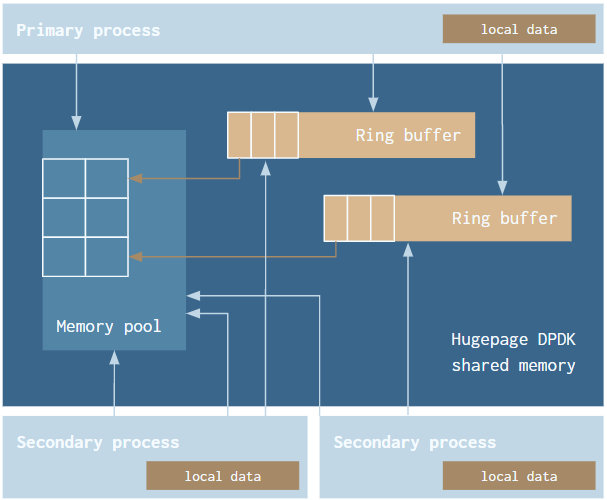
\includegraphics[width=1\textwidth, height=0.72\textwidth]{Fig5}
  \caption{Memory Sharing in the DPDK multi-process setup.}
  \label{fig:sharedmem}
\end{figure}

\section{Related work}
This section presents the existing literature that addresses issues similar to the researched ones. The idea for this thesis is based on future work sections of a few of the articles presented in this chapter.
There is a large body of recent works on measuring Docker’s performance. Overall, they can be divided into the two categories of works focusing on the offline container efficiency and on boosting Linux network performance, respectively. Also, to provide a comparison to the results presented in this thesis, works concerning NFV placement methods were researched.

\subsection{Offline container efficiency}
Most of the papers belonging to this category focus on measuring CPU consumption, RAM, and disk I/O speed. Common to these papers is that application under test are not utilizing any network functions as it would have an impact on CPU. Studied papers show a consensus that applications running in containers do not impose overheads on CPU or they are negligible. \cite{cloud_gaming_2015} used containers for deploying cloud gaming infrastructure and concluded that containers can achieve native performance when considering CPU and GPU usage. \cite{docker_hpc_2016} presented how to deploy \gls{HPC} in containers and compared Docker to Virtual Machines in the distributed software environment. Multiple CPU-heavy applications were tested using containers in \cite{genomic_pipes_2015}, to conclude that Docker has negligible impact on performance. Docker and another containerization software - Singularity were compared in \cite{docker_hpc_2018} when using multi-host and multi-core \gls{HPC} software for earthquake simulations. Singularity was found to have some startup overhead while Docker had none. Deep learning using containers was researched in \cite{deep_learning_2017} using metrics for disk IO, CPU and GPU. Some of popular orchestration tools using Docker were benchmarked in \cite{cloud_orchestration_2019}. Docker’s disk I/O performance has also been researched, but will not be mentioned since non-volatile memory does not play any role in experiments performed in this thesis.

\subsection{Linux networking stack performance}
The papers belonging to this category focus on measuring throughput and latency of packets sent, which are also the performance metrics considered in this thesis. Different from offline metrics, the applications being run inside containers usually restrict from intensive workloads to clarify the impact of network packet processing on CPU and memory. Because of that, most of the research in this area falls into the category of \gls{NFV}. A very thorough investigation of Docker network performance using different software switches was performed by \cite{anderson_2016}, which measures jitter, in addition to standard across other papers throughput and latency. The study of different hardware-agnostic packet processing frameworks to improve throughput of containers was presented in \cite{thesis_2019}. \cite{hpc_nfv_2017} compares containers' network overhead of two alternative network switches: Linux bridge and BESS. \cite{vm_vs_container_2015} compares software running in container and KVM to native implementation in a set of workloads stressing CPU, memory and network resources. It mentions \gls{NAT} as a source of overhead. \cite{big_data_2016} identifies the network I/O as a bottleneck in Big Data Environments when using containers and analyzes it.

The researchers agree that context switching and copying packets by Linux network stack are the factors that contribute to overheads the most. \cite{virt_nfv_2015} presents a preliminary benchmarking of virtualization technologies like Docker and VMs with DPDK-based switches. \cite{thesis_2017} evaluates userspace networking as a mean to accelerate Docker containers' performance. The use case of running thousands of small Network Functions on a single machine using \gls{DPDK} framework is presented in \cite{dpdk_insight_2014}. In \cite{nvf_perf_2017} different frameworks and software switches based on DPDK were evaluated. Different userspace processing frameworks like Netmap and DPDK were researched in combination with Click software in \cite{barbette_2015}. These papers show that kernel bypass is a popular movement in \gls{NFV} aiming to overcome problems related to \gls{OS}-induced overheads.

\subsection{NFV placement models}
In cloud computing, service providers rely on the flexibility given by Network Functions Virtualization to ensure that resources (services like firewalls, NATs, etc.) are allocated to the user in the most efficient manner possible. \cite{nfv_placement2} and \cite{nfv_placement3} emphasize that the way instances of different services are combined into chains plays a big part in that process. \cite{nfv_placement1} extends on that idea and considers a problem of maximizing the throughput passing through a chain of services, while \cite{nfv_placement4} considers the NFV placement as a problem of load balancing. Best to our knowledge, thoughtful placement of Network Functions on certain CPU cores based on the dynamic data rates has not yet been researched.

\cleardoublepage


\chapter{Methodology}
\label{ch:methods}

The objective in this thesis is to investigate whether using kernel bypass techniques for optimizing Docker container network communication for \gls{NFV} chains is a feasible solution. In order to answer this question, a packet-processing and analyzing system framework based on the packet processing framework \gls{DPDK} has been implemented. This chapter describes the research process and experimental design of the project. It also discusses the data collection required for the experiments, its analysis and evaluation.

\section{Research process}

In what follows we discuss scientific steps taken to conduct accurate investigation of the subject. This section is divided into the following parts: background study, design and implementation, system modeling and evaluation.

\subsubsection{Background study}

The project began with the study of topics related to the problem. Firstly, Docker containerisation was researched, followed by Linux networking stack. Then, after the initial problems were identified, the \gls{NFV} area was investigated and \gls{DPDK} framework chosen as the most viable solution for this project. The implementation idea was motivated by the conclusions and challenges presented in \cite{anderson_2016}.

\subsubsection{Design and implementation}
The implementation started with the hardware setup, consisting of two connected machines, both equipped with fast \glspl{NIC}. Then, basic implementation of the system forwarding packets through two C++ applications was created based on \gls{DPDK} example programs. After that the implementation was extended with the per-app latency measurements, context-switch time counters, throughput counters and CPU statistics. Also additional tools were set up - database for data, and visualization tools for live measurements. Finally, multi-chain and multi-app support was added. This included the \gls{DPDK} source code modifications in order to allow multiple programs per a single CPU core.

\subsubsection{System modeling}
After having the implementation in place we provided the analytical model of the considered system. In particular, we expressed the average packet latency as a function of the input data rate, the context-switch times and the number of applications competing for a CPU core. This allowed us to obtain a solid understanding of what to expect from the measurements that followed.

\subsubsection{Evaluation}
In the end, the interesting test scenarios were chosen, and relevant data gathered. Then different relationships between variables were plotted and analyzed, and the numerical results based on both the measurements and the developed analytical model were presented.

\section{Experimental design}
The project presented in this thesis mainly focuses on the following three configurable parts: applications, system configuration, and analyzer.

\begin{itemize}
    \item Applications - are parts of the system that require implementation. Their task is to perform certain work on each packet that passes through them. Each of them is embedded in separate Docker container.
    \item System configuration - specifies how the applications are connected in chains as well as their CPU core affinities. Based on this configuration the server creates shared memory sections that are used by the system.
    \item Analyzer - enables the configuration of database table where time-stamped performance metrics are stored.
\end{itemize}

In this project the workload of each application has been set to be constant. The system configuration is specified through a 2-dimentional array of \(coreNumber\)s, where the \( coreNumber \) must be in \([1, coreCount - 2]\) range as core 0 is reserved for server, and at least 1 core (the last) must be free in order to run programs such as logger, database, graphical tool, and ssh. An example of experimental configuration and resulting system layout for 8-core CPU is presented in Figure~\ref{fig:input}. Each row in the matrix represents single chain. Each number in the matrix (and rectangle in the figure) represent one application pinned to specific CPU core.

\begin{figure}
    \begin{minipage}[b]{.35\textwidth}
        \centering
        $\begin{bmatrix}
            \phantom{1}1\phantom{1} & 3\phantom{1}\\
            \phantom{1}3\phantom{1} & 4\phantom{1} & 5\phantom{1}\\
            \phantom{1}4\phantom{1} & 2\phantom{1} & 6\phantom{1}\\
            \phantom{1}6\phantom{1}
        \end{bmatrix}$
        \newline\newline\newline
    \end{minipage}
    \hfill
    \centering
    \begin{minipage}[b]{.64\textwidth}
        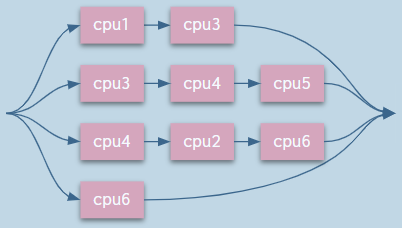
\includegraphics[width=1\textwidth]{Fig7}
    \end{minipage}
    \caption{Example of an experimental system configuration.}
    \label{fig:input}
\end{figure}


\subsection{Test environment}

Two separate machines were used to set up the environment. Both of them are a commodity hardware running Ubuntu \glspl{OS} and have been equipped with additional \glspl{NIC}. One of the machines, in the following referred to as \emph{Machine 1}, was dedicated to be the packet generator, while the other one, in the following referred to as \emph{Machine2}, was dedicated to be the packet processor. The network configuration is illustrated in Figure~\ref{fig:netconf}. Interfaces dedicated to \gls{DPDK} do not have any IP addresses assigned as they are not handled by Linux kernel. The \gls{DPDK} processes packets without interaction with layer 2 or layer 3 network, which gives the first machine's network an impression that its interfaces are connected to each other. The framework was designed with one-way packet processing in mind. However, it also passes packets back to enable protocols like ARP, TCP or ICMP between eth1 and eth2. The statistics are collected by Logger application and sent to time-series database InfluxDB. For the visualization of experiments the Grafana server is used. 

\subsubsection{System setup}
The focus in this section is on the system setup concerning Machine 2. To set up the system for the framework, the following steps must be taken:

\begin{itemize}
    \item Install \gls{DPDK} either from source or using package manager.
    \item Install Influxdb and Grafana software for statistics logging.
    \item Load uio\_pci\_generic kernel module.
    \item Use dpdk-devbind utility tool bind said kernel module to interfaces eth1 and eth2.
    \item Enable desired amount of 2MB hugepages (this project used 1024) and mount hugetlbfs file system. 
\end{itemize}

\begin{figure}[!ht]
  \begin{center}
    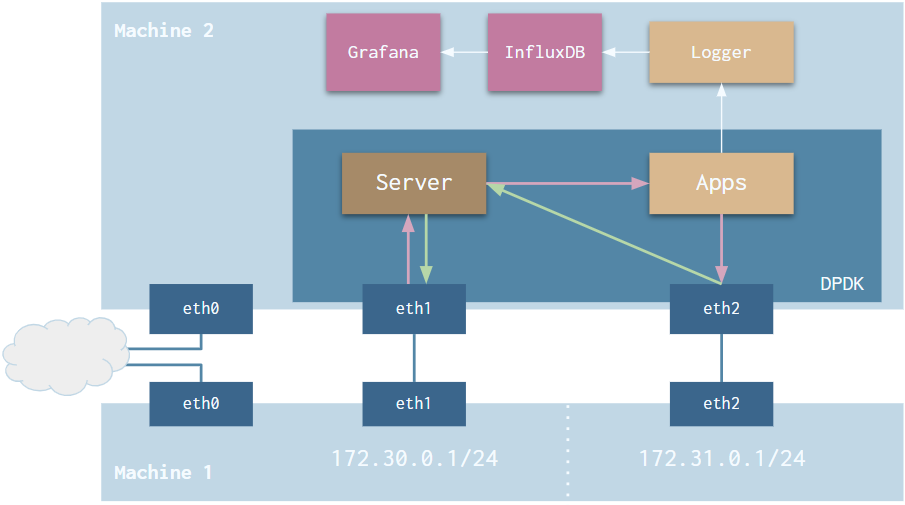
\includegraphics[width=1\textwidth]{Fig8}
  \end{center}
  \caption{Test bed used for experiments. Pink and green arrows represent traffic data travelling forward and backward through the system, respectively. White arrows represent statistical data.}
  \label{fig:netconf}
\end{figure}

\subsubsection{Hardware and software used}
The experiments were conducted on Ubuntu running on Intel Xeon CPU with 8 cores. The NIC used was Intel's 10-Gigabit Ethernet Controller with 2 ports. The machine was equipped with 32GB of RAM, of which 2GB was allocated for hugepages. Detailed hardware and software versions are presented in Table~\ref{tab:version}.

\begin{table}[!ht]
  \begin{center}
    \caption{Hardware and software used.}
    \begin{tabular}{l|r} % <-- Alignments: 1st column left, 2nd middle and 3rd right, with vertical lines in between
        \textbf{Hardware} & \textbf{Model} \\
        \hline
        CPU & Intel\textsuperscript{\textregistered} Xeon \textsuperscript{\textregistered} CPU E3-1268L v3 2.30GHz\\
        NIC & Intel\textsuperscript{\textregistered} EC 10-Gigabit X540-AT2 1528 \\
        \hline
        \textbf{Software} & \textbf{Version} \\  
        \hline
        Linux kernel & 4.15.0-96-generic\\
        DPDK & 19.11.1\\
        Docker & 19.03.7\\
        Grafana & 6.7.2\\
        InfluxDB & 1.7.10
    \end{tabular}
    \label{tab:version}
  \end{center}
\end{table}

\cleardoublepage
\chapter{System Model and Implementation}
\label{ch:whatYouDid}
This chapter provides the analytical model of the implementation and methods used to describe and predict the performance of the system.

\section{Model}
\label{sec:model}
The core idea behind the implementation is enabling the system to process multiple DPDK-enabled applications on the same CPU core, which DPDK does not support by default. Since the applications are individual processes implemented in C++, there are significant overheads imposed on the system due to context switching. When left unsupervised, the OS has a very hard time correctly switching applications to maintain their performance. This is why the implementation must decide itself when it is the correct time to yield the CPU.

\subsubsection{Switching and latency}
There has been very little study on how much time a Linux context-switch takes. \cite{switch_time} measured it to be around 1-2 microseconds when using thread pinning, which is a very short amount of time. However, this time grows on importance if switching happens very often, which is equivalent to the threads working for short periods of time. For example, if a thread is on average switched after only 10 microseconds, the switching itself becomes a major impact on the packet's latency (10-20\%), as well as the throughput capabilities of the system. Therefore, there is a need for the efficient solutions that jointly optimize the packet latency and the throughput while taking into consideration the system limitations.

To understand the main factors contributing to the latency, it is useful to take a look at the route that a single packet takes inside of the system. Figure~\ref{fig:ringbuffers} shows such a route for a single application that has one input and one output buffer ring. 

\begin{figure}[!ht]
  \begin{center}
    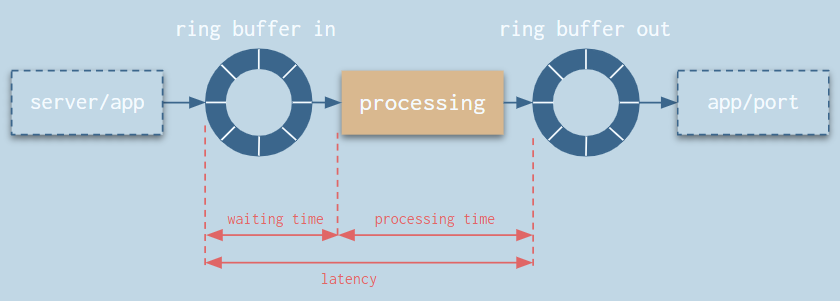
\includegraphics[width=1\textwidth]{Fig9}
  \end{center}
  \caption{Route of a packet traveling through a single application. It starts and terminates in a ring buffer.}
  \label{fig:ringbuffers}
\end{figure}

The latency of a packet caused by a single application \(T\) can be defined as a sum of the time the packet spends in the input buffer waiting for processing \(W\) and the processing time \(S\).
\begin{equation}
\label{eq:0}
T = W + S.
\end{equation} \\
As discussed in Section~\ref{userspace_pp}, one of the key optimizations implemented by DPDK is I/O batching, which means that packets are received in the constant-size arrays instead of one-by-one. However, when running many applications on a single core, the processing speed of the core must be significantly  larger than the rate at which the data arrives. Furthermore, it is important to notice that the waiting time of one application is dependent on processing times of other applications. All of this leads to the conclusion that to minimize the waiting time, the process should yield its CPU as soon as it empties the buffer.

An example of the theoretical buffer usage, as well as expected packets' waiting times for a 3-app scenario, are presented in Figure~\ref{fig:processing}.
\begin{figure}[!ht]
  \begin{center}
    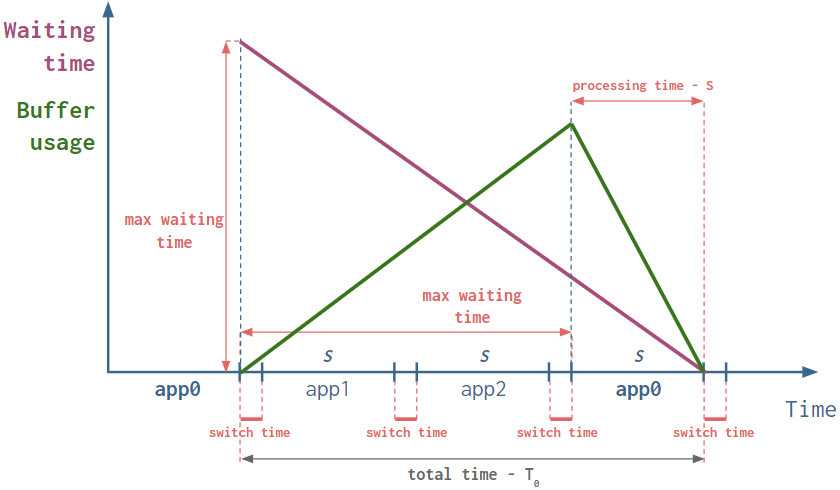
\includegraphics[width=1\textwidth]{Fig10}
  \end{center}
  \caption{Waiting time and buffer usage in time for a single application (app0) in a 3-process-1-core setup.}
  \label{fig:processing}
\end{figure}
As illustrated in the figure, the waiting time mainly depends on the factors such as processing speed, switching times and the number of applications. In what follows we model the average waiting time as a function of these parameters.

\subsubsection{Average waiting time for a single application}
We consider the packets of constant size and denote by \(W\) and \(S\) the waiting and the processing time of a single packet, respectively, and by \(T_o\) the time passed during processing the full circle of the applications. In order to express the relationship between \(W\), \(S\) and \(T_o\) in what follows we introduce the following notation:
\begin{itemize}
    \item \(x\) - the moment in time when a packet arrived in the queue.
    \item \(q(x)\) - amount of packets in the buffer at moment \(x\).
    \item \(V_1\) - the rate at which the data arrives to the buffer.
    \item \(V_2\) - processing speed
\end{itemize}
Now, the waiting time for a packet that arrived at moment \(x\) can be defined as the sum of time left till the start of processing and the time required to process already queued packets:
\begin{equation}
\label{eq:1}
\begin{split}
W(x) & = (T_o - S - x) + \frac{q(x)}{V_2} \\
       & = (T_o - S - x) + \frac{xV_1}{V_2}.
\end{split}
\end{equation}
The total amount of packets queued over \(T_o\) is equal the number of packets processed during \(S\)
\begin{equation}
\label{eq:2}
V_1 T_o = V_2 S,
\end{equation}
and thus Equation~\ref{eq:1} can be written as
\begin{equation}
\label{eq:3}
W(x) = (T_o - S) - x\left(\frac{T_o - S}{T_o}\right).
\end{equation}
The average waiting time can be calculated as follows:
\begin{equation}
\label{eq:4}
\begin{split}
\bar{W} & = \frac{\int^{T_o}_{0} W(x) dx}{T_o}\\
       & = \frac{\int^{T_o}_{0} (T_o - S) - x\left(\frac{T_o - S}{T_o}\right) dx}{T_o} \\
       & = \frac{T_o (T_o - S) - \frac{1}{2} T_o^2 \left(\frac{T_o - S}{T_o}\right)}{T_o} \\
       & = \frac{1}{2} (T_o - S).
\end{split}
\end{equation}

Next, let us denote by \(T_s\) a single switch time that includes all direct and indirect overheads between processing times of two consecutive applications, and by \(A\) the number of applications on the same core. Then, the total time \(T_o\) can be expressed as a function of \(T_s\) and \(A\) as follows.
\begin{equation}
\label{eq:5}
T_o = A (S + T_s).
\end{equation}
By substituting Eq.~\ref{eq:5} into Eq.~\ref{eq:3} we can express processing time \(S\) as
\begin{equation}
\label{eq:6}
\begin{split}
& V_2S = V_1A\left(S + T_s\right)\\
& S = T_s \left(\frac{V_1 A}{V_2 - V1 A}\right).
\end{split}
\end{equation}
Finally, it follows from Eq.~\ref{eq:5} and Eq.~\ref{eq:6} that the average waiting time in Eq.~\ref{eq:4} can be expressed as
\begin{equation}
\label{eq:8}
\bar{W}
    = \frac{1}{2}T_s\left(\frac{1 - \frac{V_1}{V_2}}{\frac{1}{A} - \frac{V_1}{V_2}}\right),
\end{equation}
where \(V_1 < V_2\) must hold for stability.\\
Figure~\ref{fig:avgwt} shows the average waiting time \(\bar{W}\) as a function of the the rate \(V_1\) at which the data arrives to the buffer. The results are shown for 5 scenarios with \(A \in \{2,3,4,5,6\}\), respectively for constant values of \(T_s = 1 [us]\) and \(V_2 = 5000 [Mbits/s]\). We can observe that the closer \(V_1\) is to  \(V_2\) the higher its impact on \(\bar{W}\). We can also notice that if the ratio of \(V_1/V_2\) is lower than around 0.8, the number of applications \(A\) has little impact on average waiting time \(\bar{W}\). This could be a useful information if a real-life deployment of such system was considered.
\begin{figure}[!ht]
  \centering
    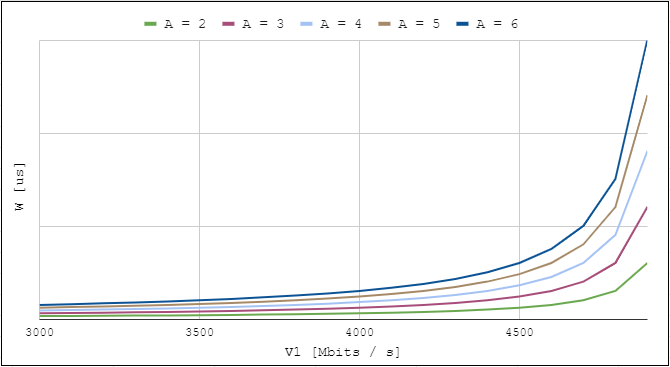
\includegraphics[width=1\textwidth]{Fig12}
  \caption{Average waiting time \(\bar{W}\) of a single packet (1.6kbit) vs. the rate \(V_1\) at which the data arrives to the buffer.}
  \label{fig:avgwt}
\end{figure}
\subsubsection{Mean performance metrics}
\label{sec:expectations}
Observe that the average waiting time \(\bar{W}\) depends on four parameters, that is, \(V_1\), \(A\), \(T_s\) and \(V_2\) (c.f., Equation~\ref{eq:8}), where parameters \(V_1\) and \(A\) are determined by the user, while parameters \(V_2\) and \(T_s\) characterize the system and the implementation of the applications.
The time of a single switch \(T_s\) and the overheads that accompany it, in theory, should not be affected by either input data rate \(V_1\) or the number of applications \(A\). This is due to applications being instances of the same program and the processed data being stored in the shared memory.
The processing speed \(V_2\) is also expected to be constant as it depends only on the uninterrupted performance of the CPU. However, it might be slightly lower for small data rates due to the nature of I/O batching. That is because whenever the application polls for a new batch of packets, it asks for a constant-size buffer. A situation in which the application receives a lower amount of packets than the buffer size can contribute to lower processing speed as the poll itself is a significant cost. The relationship between the processing speed \(V_2\) and the number \(q\) of packets queued for processing can be expressed as
\begin{equation}
\label{eq:9}
V_2(q) = \frac{q}{ceil\left(\frac{q}{S}\right)T_{poll} + qT_{proc}},
\end{equation}
where \(S\) is size of the buffer, \(T_{poll}\) time of single poll and \(T_{proc}\) time of actual processing. This equation gives us the processing speed given that the amount of packets queued at the moment of processing is always exactly \(q\). However, this is not the case as packets arrive with some random distribution. To take that into account, variable \(R\) was used as the amount of polls the software must do to empty the buffer \(ceil\left(\frac{q}{S}\right)\). Let us also define \(\overline{q}(R)\) as an average number of packets received, when R polls occur:
\begin{equation}
\label{eq:9.5}
\overline{q}(R) = \frac{\sum_{S(R-1)}^{SR} i}{S} = S(R-\frac{1}{2}).
\end{equation}
This equation expresses a situation when the last poll always fills half of the buffer. Therefore, Equation~\ref{eq:9}, when substituted with Equation~\ref{eq:9.5} presents a more aggregated model of processing speed \(V_2\), more likely to be observed during measurements:
\begin{equation}
\label{eq:10}
V_2(R) = \frac{S \left(R - \frac{1}{2}\right)}
           {RT_{poll} + S \left(R - \frac{1}{2}\right)T_{proc}}.
\end{equation}
Figure~\ref{fig:v2graph} shows \(V_2(q)\) and \(V_2(R)\) as a function of queue size \(q\) for \(S = 8\). We can see that the low amount of packets in the queue at the start of processing can hurt performance of the system using I/O batching.

\begin{figure}[!ht]
  \centering
    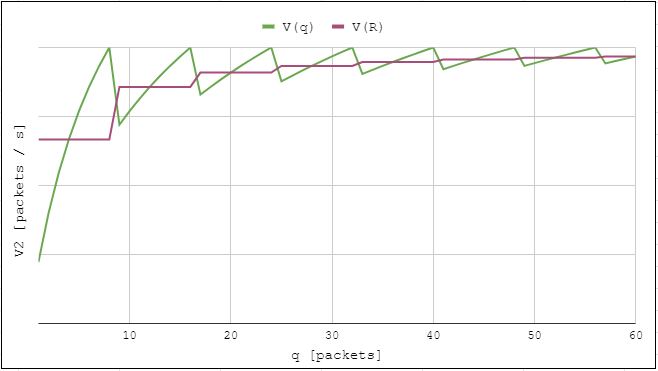
\includegraphics[width=1\textwidth, height=0.5\textwidth]{Fig11}
  \caption{Relationship between processing speed \(V_2\), number of packets queued \(q\), and number of polls \(R\).}
  \label{fig:v2graph}
\end{figure}

\section{Performance metrics}
To evaluate the performance of packet processing during the tests, the focus was on the following performance metrics:

\begin{itemize}
    \item Latency - the precise (recorded in microseconds) latency created by each network element is measured. The server includes a timestamp into the packet's metadata immediately after receiving it from input port. Then, right before sending it to the next application, the accumulated latency is measured and stored. Since saving the latencies of each packet would be infeasible, they are averaged over a period of time.
    \item Throughput - the amount of data each application processes per second. The throughput is measured taking into account whole Ethernet packets' sizes.
    \item CPU consumption - the percentage of time the CPU spends in each mode. The measurements are performed separately for each core. Since DPDK processes will always attempt to make use of whole free processing power, the most important statistic is the time spent in userspace compared to time spent in kernel space.
\end{itemize}

\section{Implementation}
This section presents interesting and important parts of the software implementation, showing mechanisms like ring/port communication, context-switch management, packet processing, and explaining how the measurements are performed and collected.

\subsubsection{Communication}
DPDK provides two mechanisms for receiving and sending packets: ports - the endpoints of the system, and ring buffers - used for inter-app communication. Both of these mechanisms operate on structures called \(mbufs\), which are provided by DPDK. A single \(mbuf\) stores packet's data and metadata in one place. Every poll either from port or ring requires passing a preallocated array of \(mbufs\). The abstraction used for that is shown in Figure~\ref{fig:code1}.
\begin{figure}[!ht]
\begin{code}[language={C}, label=lst:mbuffer]
struct MBuffer
{
    static const int CAPACITY = 8;
    uint size;
    
    rte_mbuf* data[CAPACITY];
    rte_mbuf* operator [] (int index) 
    { 
        return data[index]; 
    }
};
\end{code}
\label{fig:code1}
\caption{Abstraction for a buffer of DPDK's rte\_mbufs.}
\end{figure}

To simplify the data flow in the code, both port and ring were implemented as classes and generalized to a \(Device\). The C++ implementation for the \(Device\) is presented in Figure~\ref{fig:device}. 
\begin{figure}[!ht]
\begin{code}[language={C}]
class Device
{
public:
    Device(int chainIndex, int appIndex);

    virtual void getPackets(MBuffer &buffer) = 0;
    virtual int sendPackets(MBuffer &buffer) = 0;

protected:
    // Position in the system
    int _chainIndex;
    int _appIndex;
};
\end{code}
\caption{Device class - a generalization of Port and Ring classes.}
\hspace*{2in}
\label{fig:device}
\end{figure}
Passing data from one \(Device\) to another is done by a \(Sender\) class. It is also tasked with recording statistics and invoking a user-programmed callback for each packet. The relationship between classes in the implementation is shown in Figure~\ref{fig:classdiagram}.
\begin{figure}[!ht]
  \centering
    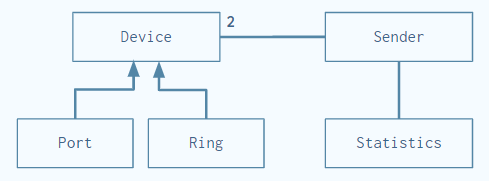
\includegraphics[width=0.8\textwidth]{Fig13.png}
  \caption{Class diagram showing basic relationship of entities in the library.}
  \label{fig:classdiagram}
\end{figure}

\subsubsection{CPU affinities}
To make the context-switching as reliable as possible, all the CPU affinities of all programs running on the machine must be controlled. DPDK implements that feature as part of the library, so the affinities of the server and applications can be easily controlled by passing an argument. One of the hard requirements of DPDK is that although there can be many programs running on the same core, the maximum amount of programs is the same as the core count. To mitigate that restriction, we first identified that the function \(rte\_eal\_cpu\_init(void)\) limits the number of threads and assigns their default affinities. Then, we modified the function such that the specific affinities can be set using the built-in \(lcores\) argument. The output of starting script is presented in Figure~\ref{fig:script}.\\

\begin{figure}[!ht]
\begin{code}
./build/server --lcores=0@0 -- 1 1 1
./build/app    --lcores=1@1 --proc-type=auto -- 0 0
./build/app    --lcores=2@1 --proc-type=auto -- 1 0
./build/app    --lcores=3@1 --proc-type=auto -- 2 0
\end{code}
\caption{Commands used to start a server and 3 applications in 3 separate chains. The \(lcores\) argument takes two values: uniqueID@coreIndex. This results in the server running on core 0 and 3 applications running on core 1.}
\label{fig:script}
\end{figure}
Having DPDK programs under control, we then set the affinities of all the other applications running on the system in a way that prohibits them from using the DPDK-designated cores. Although a more advanced strategy would be useful in an enterprise deployment, for the purpose of tests a simple taskset command, as presented in Figure~\ref{fig:taskset}, proved to be sufficient.
\begin{figure}[!ht]
\begin{code}
for i in $(ps -e -T -o pid | awk '{print $1}')
do
    taskset -a -p -c 4-7 $i
done
\end{code}
\caption{Taskset command used to set the affinities of all the programs and their threads running on the machine to CPU cores 4-7.}
\label{fig:taskset}
\end{figure}

\subsubsection{Context-switching}
After assigning all the affinities, let us look at the switching between applications. To make sure that the amount of context switches is controllable, each application uses the switching algorithm SCHED\_FIFO. This disables the scheduler's time slicing, ensures that the apps are always granted CPU in the same order, and allows them to run until they yield, using \(sched\_yield()\). This is also why re-pinning the other programs to free cores is important, as SCHED\_FIFO forbids any applications with default scheduling to run, making them starve. The corresponding code as well as mechanisms described in the Model section allowing the app to run until it empties the buffer, are shown in Figure~\ref{fig:switching}.

\begin{figure}[!ht]
\begin{code}
sched_param sp = { .sched_priority = 1 };
pthread_setschedparam(pthread_self(), 
                      SCHED_FIFO, 
                      &sp);

// Time for other apps to set scheduling
sleep(3);

// Main app loop
for (;;)
{
    const int c = sender->sendPacketBurst();

    if(c < MBuffer::CAPACITY)
    {
        // ...
        sched_yield();
    }
}
\end{code}
\caption{Scheduling and priority configuration, main app loop.}
\label{fig:switching}
\end{figure}

\subsection{Measurement techniques}
To obtain variables required to model the behaviour of the system, different measurements are gathered during run-time. The following statistical data are collected per application:
\begin{itemize}
    \item number of switches,
    \item number of polls between switches,
    \item time between receiving and yielding CPU,
    \item time spent waiting for CPU,
    \item time each packet spends waiting for processing,
    \item CPU time spent in user mode,
    \item number of bytes processed.
\end{itemize}
The block diagram in Figure~\ref{fig:blockdiagram} presents the functioning of an application's processing loop. It does not include CPU measurements as they are collected independently from the system statistics. In the figure the left column shows the processing of a single batch of packets. We can see that timestamps T1 and T2 are taken only once for a buffer of packets. This was required to reduce the influence of time capturing on the performance of the processing, which is the most time-sensitive part of implementation.

\begin{figure}[!ht]
  \centering
    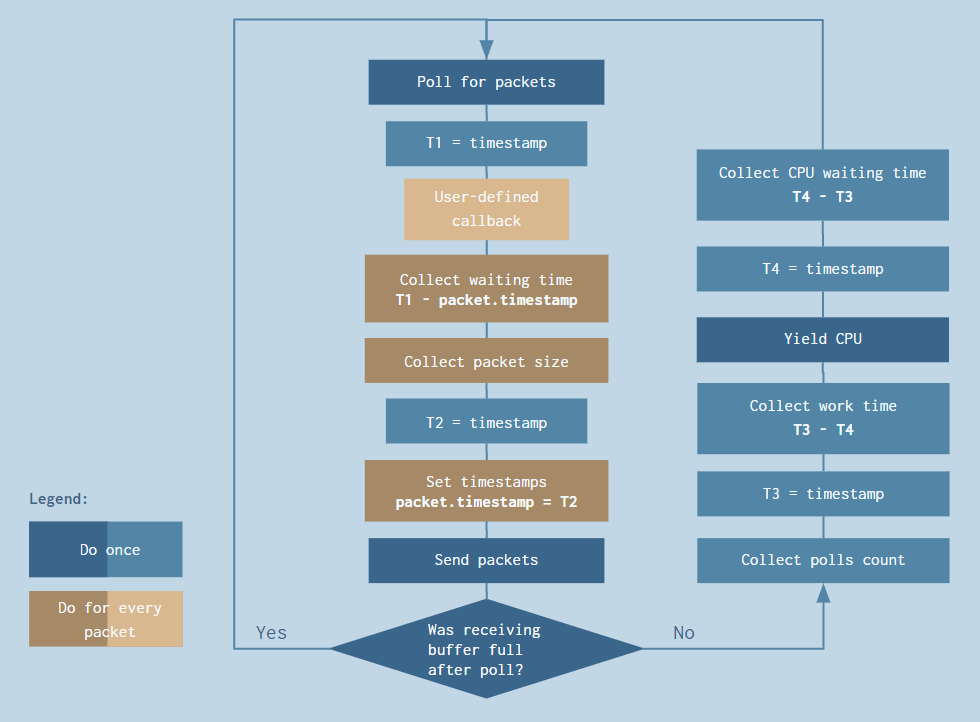
\includegraphics[width=1\textwidth]{Fig14.png}
  \caption{Block diagram showing the work process of application including data collection.}
  \label{fig:blockdiagram}
\end{figure}

\subsubsection{Instrumentation}
Finally, the technique of statistic collection plays an important role in minimizing the overheads of the system analysis. The statistics are gathered over a time period of 1 second, then averaged, and sent further to be filed. Tests showed that it is infeasible to write the data to the file or send over HTTP, hence all of the applications share a multi-producer ring buffer. On the receiving side, there is a logger program gathering all the messages sent by apps and forwarding them to the database. Even though the logger is a DPDK-enabled program, it is not CPU dependent. In that it can use mechanisms like sleeps and work outside the affinity-shielded cores.

\subsection{Test configuration}
The following configurations were chosen to verify the claims presented in previous sections. The system was set up with one layer of parallel applications, all running on the same CPU core, with workload set to 1. The server and logger were running on separate cores. The traffic generated by MoonGen application was set to produce UDP packets of 200 bytes size. The buffer capacity of the applications was set to 8. The tests have been performed for scenarios with \(A \in \{2,3,4,5,6\}\) and \(V_1 \in [3,8] Gbit\). The components of the corresponding test bed are illustrated in Figure~\ref{fig:testbed}. It presents the server running on core 0, all applications on core 1, and logger on core 2.

\begin{figure}[t]
  \centering
    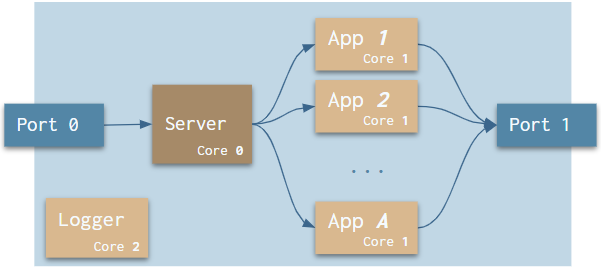
\includegraphics[width=1\textwidth]{Fig15.png}
  \caption{Test configuration of the system used for analysis, with one layer of similar applications with a  similar workload.}
  \label{fig:testbed}
\end{figure}

\cleardoublepage
\chapter{Results and analysis}
\label{ch:resultsAndAnalysis}
In this chapter we present the results obtained using the methods described in Chapter~\ref{ch:methods} and the results obtained for the model developed in Chapter~\ref{ch:whatYouDid}, respectively.

\section{Switch Time and Processing Speed}
We start with evaluating switch time \(T_s\) and processing speed \(V_2\) as a function of \(V_1\). The results are shown for five different scenarios with \(A \in \{2,3,4,5,6\}\).

\subsubsection{Switch Time}
Figure~\ref{fig:switchtime} shows the average time of a single switch depending on the number of applications \(A\) and input data rate \(V_1\). Although the switch time \(T_s\) was expected to be constant and independent of neither \(A\) nor \(V_1\) as discussed in Section~\ref{sec:expectations}, the results show the opposite. We observe that for the number of applications \(A > 2\) the gap between measured switch times is almost negligible and it increases with \(V_1\). One explanation of such behaviour would be that as the data rate increases, the amount of time it takes to flush a \gls{TLB} increases as well. On the contrary, the switch time is significantly smaller for \(A = 2\) and it only rises slightly as \(V_1\) increases. Both of the observed behaviours might be a result of cache misses. One explanation could be that 2 running applications can still use the cache efficiently, while running 3 or more causes cache perturbation and in effect denies cache usage. The problem of cache misses related to context switching has been well reviewed in \cite{context_switch_cache}.

\begin{figure}[!ht]
  \centering
    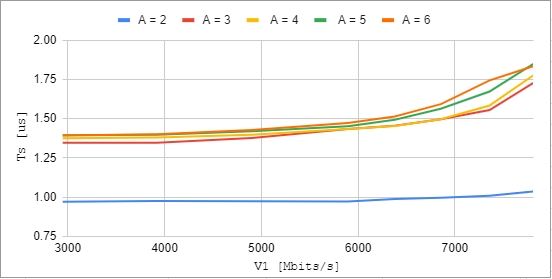
\includegraphics[width=1\textwidth]{Fig16.png}
  \caption{Relationship between average time of a single context switch \(T_s\), number of applications \(A\) and incoming data rate \(V_1\).}
  \label{fig:switchtime}
\end{figure}

\subsubsection{Processing Speed}
The processing speed \(V_2\) of a single application has been presented in the Figure~\ref{fig:v2result}. In the figure we can observe that the processing speed slowly rises with input data rage \(V_1\), which we conclude is a result of I/O batching, as described in Section~\ref{sec:expectations}. At the same time it does not seem to depend on the number of applications \(A\), as results related to different \(A\)s but same \(V_1\) are always very close to each other.
\begin{figure}[!ht]
  \centering
    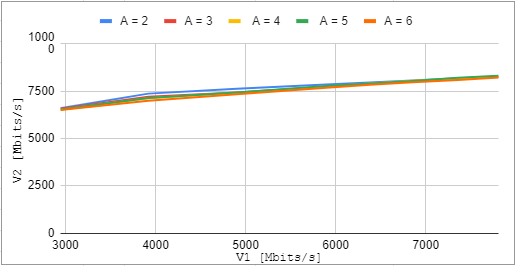
\includegraphics[width=1\textwidth]{Fig17.png}
  \caption{Relationship between the processing speed \(V_2\) of a single application, number of applications \(A\) and incoming data rate \(V_1\).}
  \label{fig:v2result}
\end{figure}

\section{Waiting time}
In Figure~\ref{fig:Twresults} we show the results obtained from the measurements (solid line) and the results obtained using the model presented in Section~\ref{sec:model} (dashed line), respectively. The results show that the average waiting time \(\bar{W}\) increases as the data arrival rate \(V_1\) increases. Furthermore, we observe that the gap between the results obrained from the measurements and the model based results is small in all scenarios, which confirms that the model proposed in Section~\ref{sec:model} successfully captures the behaviour of the considered system. In the figure we can see that both measured and modelled results behave in a similar way.
\begin{figure}[!ht]
  \centering
    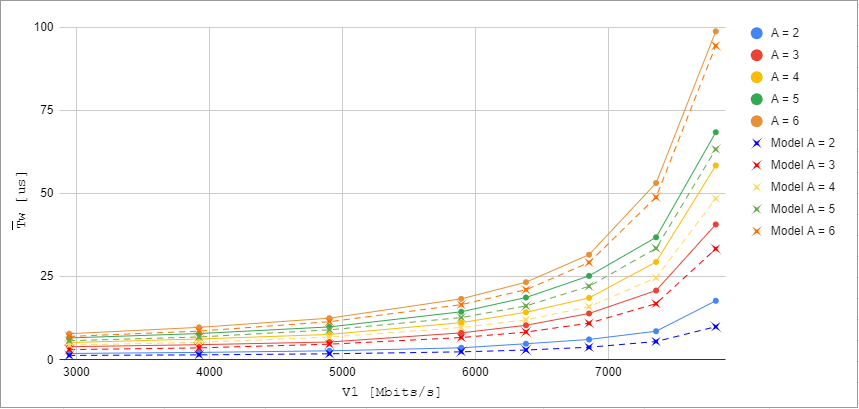
\includegraphics[width=1\textwidth]{Fig18.png}
  \caption{Relationship between the average waiting time \(\bar{W}\), number of applications \(A\) and incoming data rate \(V_1\). Solid lines show measured waiting time, while dashed lines show the time calculated using model.}
  \label{fig:Twresults}
\end{figure}
The gap could be explained by the fact that in the case of results obtained from measurements the timestamps for waiting times were saved before the \(send()\) and after the \(receive()\) functions, which can themselves add small overheads to the elapsed times. Another factor that might contribute to observed differences might be the fact that switching time is a very influential factor in the model and even a small discrepancy in the measurements might produce noticeable differences. The latter is especially likely to happen in the case of a busy loop, where the overhead added by the measurements may be significant.

\subsubsection{Ratio of waiting times}
In order to get insights into how the gap between the measurement and model based results depend on the values of \(A\) and \(V_1\), let us denote by \(\bar{W}^{measurement}\) and \(\bar{W}^{model}\) the average waiting times obtained from the measurements and using the model, respectively and let us denote the ratio of the two by C:
\begin{equation}
C = \frac{\bar{W}^{measurement}}{\bar{W}^{model}}
\end{equation}
Figure~\ref{fig:missingC} shows ratio \(C\) as a function of the number of applications \(A\) for different values of \(V_1\). We can observe that \(C\) is slightly affected by the change in the values of \(V_1\) and mostly affected by the change in the values of A. The difference between the results obtained for different values of V1 is most noticeable for \(A=2\), and the gap between the results vanishes as \(A\) increases. We also observe that the ratio \(C\) decreases as \(A\) increases for all values of \(V_1\) and already for \(A = 6\) it reaches the values close to 1. These results suggest that the the model presented in Section~\ref{sec:model} is especially suitable for the systems with medium to large numbers of applications.
\begin{figure}[!ht]
  \centering
    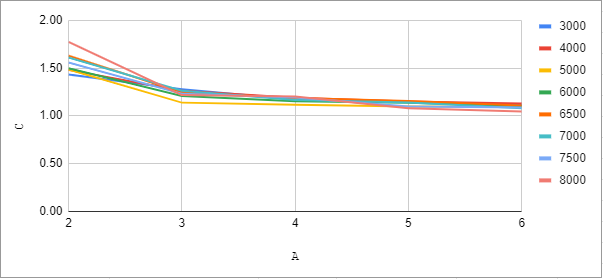
\includegraphics[width=1\textwidth]{Fig19.png}
  \caption{Relationship of the ratio \(C\), number of applications \(A\) and input data rate \(V_1\).}
  \label{fig:missingC}
\end{figure}
% Described behavior can be modeled with the following equation:
% \begin{equation}
% \label{eq:11}
% AvgC(A) = \frac{A}{A - m},
% \end{equation}
% where \(m\) is appropriately chosen constant. The \(C\) as a function of \(A\) has been fitted with this equation in  Figure~\ref{fig:fittedC}, using average values from the results presented in Figure~\ref{fig:missingC}.
% \begin{figure}[!ht]
%   \centering
%     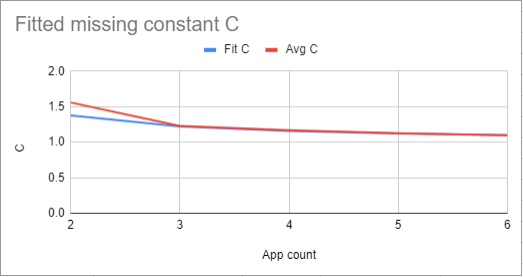
\includegraphics[width=1\textwidth]{Fig20.png}
%   \caption{Average and fitted \(C\) as functions of \(A\). }
%   \label{fig:fittedC}
% \end{figure}\\
% This resulted in \(m = \frac{1}{2}\). By multiplying \(\frac{A}{A-1/2}\) with Equation~\ref{eq:8} we can produce precise projections of the average waiting times \(\bar{T}_s\) of the system.

% \subsubsection{Use case}
% The use case requires pre-measuring of the behaviour of both switch times \(T_s\) and processing speeds \(V_2\) using any \(A\). Since both mentioned factors are not influenced by \(A\), it is possible to forecast the latencies appearing in the system for any specific \(V_1\). An example of such prediction for \(A = 6\) and \(V_1 \in [3, 8] Gbit\) using data collected for \(A = 5\) are presented in Figure~\ref{fig:fitted6model}.
% \begin{figure}[!ht]
%   \centering
%     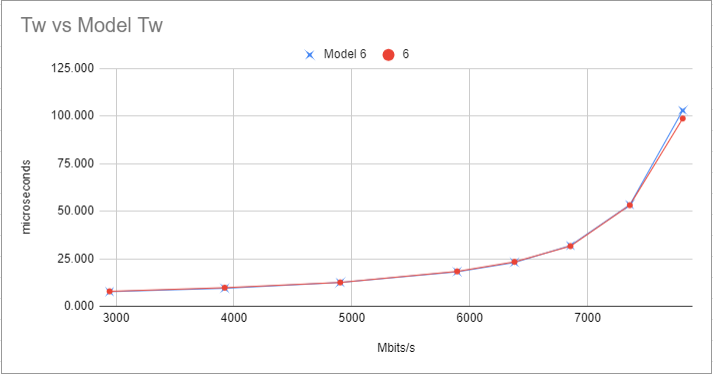
\includegraphics[width=1\textwidth]{Fig21.png}
%   \caption{Comparison of predicted and measured \(\bar{T}_s\) for \(A = 6\).}
%   \label{fig:fitted6model}
% \end{figure}

\cleardoublepage
\chapter{Conclusions and future work}
\label{ch:conclusionsAndFutureWork}
This chapter summarizes conclusions drawn from the work accomplished during this project, and emphasizes some of the interesting observations. It also describes potential future work and sustainable and ethical concerns.

\section{Conclusions}
While the NFV industry is constantly growing, it faces many challenges on the way. In this thesis we focused on the challenges regarding running dozens of containerized network functions on a single machine. To get insights into the problem we completed the goals described in the Section~\ref{sec:motivation}:
\begin{itemize}
    \item We conducted a thorough review of a significant body of papers concerning NFV, containerization, Linux networking, and fast packet processing.
    \item We created a framework shifting whole container communication into the userspace.
    \item We implemented an efficient DPDK-based system allowing for precise measurements on Gigabits of passing data.
    \item We provided an analytical model of the system and performed the measurements on the testbed that we built for the purposes of this project. 
    \item Finally, we compared the results obtained from the measurements with the results obtained using the proposed analytical model.
\end{itemize}

The project showed that it is possible to efficiently run a high number of containers performing packet processing on a single machine. It also showed that it is possible to predict the behaviour of the system in terms of the packets' latency based on few non-invasive performance measurements.

This project provided important insights into the possibilities and potential problems of cloud packet processing. It showed the importance of correct between-process-switching and its influence on the performance of the system, together with interesting behaviour regarding context-switch times on Linux. It also showed that using kernel bypass techniques is a valid option for implementing inter-container communication, and that it is possible to modify DPDK to support multiple processes on a same core.

\section{Future work}
\label{sec:futureWork}

In this section we describe future work that could improve the project, as well as potential directions for future engineers who would like to follow up on the subject.

\subsubsection{Project improvements}

Due to the limited resources, the implementation of this project was only tested on a single pair of machines. In order to further validate the model presented in the thesis, the tests should be repeated on the machines with different CPU architectures and different Linux distributions. The comparison of the context-switch behaviour would be an interesting issue to explore, as it might be influenced by the cache sizes, which vary on different CPUs.

Another useful result would be to substitute the real-life packet processing applications in place of the mock. The differences might for example occur due to the different packet sizes or the internal packet processing techniques. Following that idea, the model could be extended with the calculations for different applications running on same core.

Finally, it would be interesting to see how running the framework using multiple cores simultaneously would affect the performance results. Also, running the applications in different configurations (e.g. multi-app chain on one core), would give insights about more production-ready behaviour of the system.

\subsubsection{Future research}

This project showed that one of the factors having the most influence on the performance of packet processing is the context-switch time. Having understood that, the proper continuation of the research would be on the topic of better cache usage for this specific purpose. Cache seems to be a very important topic in DPDK development, however, the library is not created in the many-app-per-core support in mind. In our opinion the research in this direction could greatly improve the capabilities of DPDK.

\section{Reflections}
This project focused on improving efficiency of packet processing by putting several NFV applications on a single CPU core. Such a solution could potentially improve the cost-efficiency of the system and help to remove the middleboxes in lieu of cheaper common hardware substitutes. This in turn, could help start-ups and small-budget companies.

Another positive aspect of this work is that by increasing processing efficiency, it decreases the energy consumption required for the same amount of computation. The slowdown in the growth of electricity consumption in the information and communications technology (ICT) systems is of great importance as ICT systems accounted in 2012 for about 4,7\% of the electricity consumption worldwide \cite{energy_consumption}, and that value is constantly growing.

In conclusion this project does not raise any ethical concerns, but could instead improve the functioning of today's networks. 


\cleardoublepage
% Print the bibliography (and make it appear in the table of contents)
%\printbibliography[heading=bibintoc]
% The lines below are for BibTeX
\bibliographystyle{myIEEEtran}
\renewcommand{\bibname}{References}
\addcontentsline{toc}{chapter}{References}
\bibliography{references}


\label{pg:lastPageofMainmatter}
\afterpage{\blankpage}
\includepdf[pages={2}]{cover.pdf}
\clearpage
\section*{For DIVA}
\divainfo{pg:lastPageofPreface}{pg:lastPageofMainmatter}
\end{document}
